\begin{exercise}{Navier-Stokes}{10}
  Ein zylinderförmiger Stab mit Radius $R_1$ bewegt sich mit der Geschwindigkeit $u$
  parallel zu seiner Achse in einem zu ihm koaxialen zylinderförmigen Rohr mit Radius
  $R_2$. Der Raum zwischen dem Stab und dem Rohr ist mit einer inkompressiblen
  Flüssigkeit gefüllt. Die Strömung ist stationär.\\
  Wählen Sie an das Problem angepasste Zylinderkoordinaten $(r, \theta, z)$. Sie
  können davon ausgehen, dass die Geschwindigkeit $\vec{v}$ der Flüssigkeit nur von
  dem radialen Abstand von der Symmetrieachse abhängt und immer in $z$-Richtung zeigt.

  \begin{enumerate}
    \item Welche Gleichung für $v_z$ erhalten Sie ausgehend von der Navier-Stokes-Gleichung?
    \item Welche Randbedingungen gelten? D.h. geben Sie $v_z(r = R_1)$ und $v_z(r = R_2)$ an.
    \item Lösen Sie die Navier-Stokes-Gleichung für diesen Fall. D.h. berechnen Sie $v_z(r)$.
  \end{enumerate}
  
  \begin{figure}[h]
    \centering
    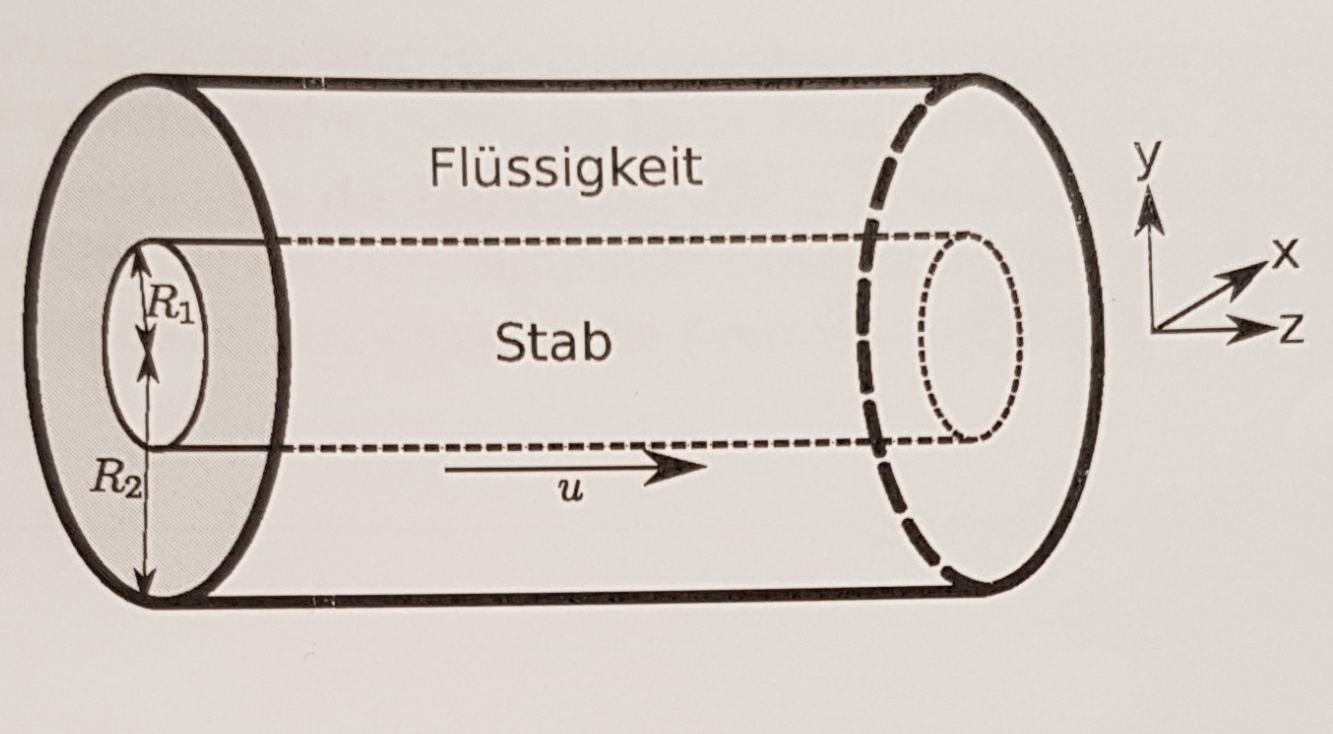
\includegraphics[width=0.7\textwidth]{Skizze_Navier_Stokes.jpg}
    \label{fig:Skizze_Koaxial}
  \end{figure}

\end{exercise}
